% 第5章第6节：树分解上的动态规划（局部函数的分配、接口表与袋消息、配置恢复与开销、计数与加权求和、半环）。

\section{树分解上的动态规划}
\label{sec:graph-bag-dp}

有了一个已经核验的树分解，就可以把第~\ref{sec:graph-tree-dp}节树上的递推搬到袋组成的树上：原来每个顶点是一个变量，现在每个节点是一组变量；原来消息以单个接收变量为索引，现在以相邻两袋的接口为索引。本节先说明局部函数怎样分配到袋中，再给出袋之间的消息递推及其正确性，然后讨论配置恢复和计算开销；最后保持同样的结构，把“相加后取最小”换成其他运算，得到可行配置计数和加权求和。

本节的例子仍是四变量问题：树分解有两个节点$s,t$，袋为$B_s=\{1,2,3\}$与$B_t=\{2,3,4\}$，接口为$\{2,3\}$；局部函数$\phi_A,\phi_B$由表~\ref{tab:graph-dp-ternary-tables}给出。

\subsection{局部函数的分配}

\paragraph{每个函数恰好归入一个袋}
计算前先把每个局部函数$\phi_a$归入一个袋$B_{\alpha(a)}$，要求$S_a\subseteq B_{\alpha(a)}$；由引理~\ref{lem:graph-dp-clique-in-bag}，这样的袋总存在。每个函数只归入一次。节点$t$上全部归入函数之和称为袋成本：
\begin{equation}
\Phi_t(\bm x_{B_t})=\sum_{a:\,\alpha(a)=t}\phi_a(\bm x_{S_a}),
\label{eq:graph-dp-bag-cost}
\end{equation}
没有函数归入的袋取$\Phi_t\equiv0$，但仍保留袋中的变量，因为它们可能需要经过这个袋来保持一致。在例子中，$\phi_A$只能归入$B_s$，$\phi_B$只能归入$B_t$，于是$\Phi_s=\phi_A$、$\Phi_t=\phi_B$。

只归入一次是数值正确性的要求，不是结构上的要求。设问题中另有一个成对项$\phi_{2,3}(x_2,x_3)$，它的作用域同时被$B_s$和$B_t$包含，归入哪个袋都可以；但若两边各计一次，最后得到的就是$F+\phi_{2,3}$的最小值，而不是$F$的最小值。共享变量可以在多个袋中重复出现，同一个成本项却不能在多处重复累计。

\paragraph{分配清单的核对}
计算前可以对照一份分配清单逐项检查：每个局部函数都有归属，没有遗漏；没有函数被归入两个袋；每个函数的作用域确实包含在所归入的袋中。树分解的三个条件只保证有地方容纳每个函数，这份唯一归属则保证每一项成本恰好计算一次。袋之间的交集只说明哪些变量需要协调，它本身不对应任何成本，不能当作额外的局部函数加入。

\subsection{接口表与消息递推}

\paragraph{袋之间的消息}
设节点$s,t$在袋树中相邻，接口为$S_{s,t}=B_s\cap B_t$。从$s$发往$t$的消息是一张以接口变量为索引的表：固定接口取值后，把袋成本与$s$从其他邻居收到的消息相加，再对$B_s$中不属于接口的变量取最小，
\begin{equation}
\mu_{s\to t}(\bm x_{S_{s,t}})=\min_{\bm x_{B_s\setminus S_{s,t}}}\Bigl[\Phi_s(\bm x_{B_s})+\sum_{r\in N(s)\setminus\{t\}}\mu_{r\to s}(\bm x_{S_{r,s}})\Bigr],
\label{eq:graph-dp-bag-message}
\end{equation}
其中$N(s)$是$s$在袋树中的邻居。这与式~\eqref{eq:graph-dp-tree-message}的结构相同，只是被汇总的不再是单个变量，而是袋内的非接口变量。

在例子中，$s$是叶节点，它的非接口变量只有$x_1$，所以
\[
\mu_{s\to t}(x_2,x_3)=\min_{x_1}\phi_A(x_1,x_2,x_3).
\]
图~\ref{fig:graph-dp-bag-message-table}逐行列出了这张四项表：接口取值为$00,01,10,11$时，消息值依次为$0,0,1,2$，达到最小值的$x_1$依次为$1,0,1,1$。它与上一节消去$x_1$得到的$\psi_1$相同。$x_1$已经被汇总，不再出现在表中；$x_2,x_3$作为接口仍然显式保留，右袋读取这张表时要按同样的$(x_2,x_3)$取值对齐。

\begin{figure}[!htb]
  \centering
  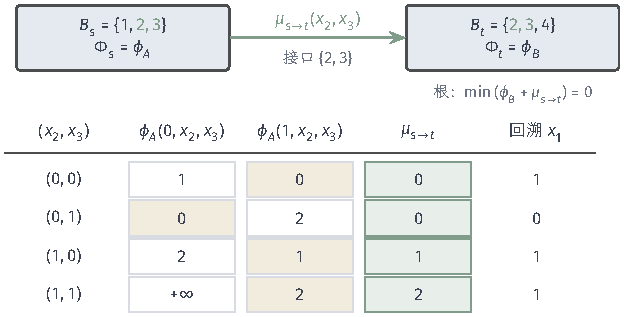
\includegraphics[width=105.650mm]{figures/01-basic-mathematics/04-graphs/tikz/c5-bag-message-table/figure.pdf}
  \caption{两袋之间的消息。左袋$B_s=\{1,2,3\}$只含$\phi_A$，右袋$B_t=\{2,3,4\}$只含$\phi_B$，接口为$\{2,3\}$（绿色）。下方表格对接口的每种取值比较$x_1=0,1$两个候选，取较小者作为消息值，黄色格是被选中的候选；绿色列是消息值，最后一列是回溯表。根袋$B_t$把消息与$\phi_B$相加后对$x_2,x_3,x_4$取最小，得到最优值$0$。}
  \label{fig:graph-dp-bag-message-table}
\end{figure}

选$t$为根，根处合并袋成本与全部入消息，再对根袋的全部变量取最小：
\[
\min_{x_2,x_3,x_4}\bigl[\phi_B(x_2,x_3,x_4)+\mu_{s\to t}(x_2,x_3)\bigr]=0,
\]
在$(x_2,x_3,x_4)=(0,1,0)$处达到，因为$\phi_B(0,1,0)=0$且$\mu_{s\to t}(0,1)=0$，而所有值都非负。一般情形下按后序计算：每个节点收齐子节点的消息后向父节点发送消息，最后在根处合并。

\paragraph{为什么沿袋树计算是正确的}
树上消息的正确性依赖于一件事：删去一条边后，两侧除了接收变量以外没有共同的变量。袋树上，这件事由运行交集保证。删去袋树边$\{s,t\}$后，袋树分成两部分；记$s$一侧全部袋中出现的变量为$V_{s|t}$，$t$一侧为$V_{t|s}$。若某个变量$v$在两侧都出现，从它在$s$侧的某个出现位置到$t$侧的某个出现位置，袋树路径必须经过边$\{s,t\}$，由运行交集，$B_s$与$B_t$都含$v$。所以
\begin{equation}
V_{s|t}\cap V_{t|s}\subseteq S_{s,t},
\label{eq:graph-dp-interface-separation}
\end{equation}
即接口把两侧的变量隔开：固定接口取值后，两侧的其余变量互不重叠，可以分别求最小。

\begin{theorem}[袋消息的含义]
\label{thm:graph-dp-bag-message}
设$(\mathcal T,\{B_t\}_{t\in T})$是原始图的树分解，每个局部函数恰好归入一个包含其作用域的袋。对袋树的边$\{s,t\}$，记$A_{s|t}$为归入$s$一侧各袋的局部函数。则对每个接口取值$\bm x_{S_{s,t}}$，
\[
\mu_{s\to t}(\bm x_{S_{s,t}})=\min_{\bm x_{V_{s|t}\setminus S_{s,t}}}\ \sum_{a\in A_{s|t}}\phi_a(\bm x_{S_a}).
\]
进一步，对任意根节点$\rho$，$\min_{\bm x}F(\bm x)=\min_{\bm x_{B_\rho}}\bigl[\Phi_\rho+\sum_{r\in N(\rho)}\mu_{r\to\rho}\bigr]$。
\end{theorem}

\begin{proof}
对$s$一侧的节点数归纳。设$s$在$t$以外的邻居为$r_1,\ldots,r_k$（叶节点时$k=0$）。删去$s$后，$s$一侧的其余节点分成$r_1,\ldots,r_k$各自的一侧。由式~\eqref{eq:graph-dp-interface-separation}应用于边$\{r_j,s\}$，$V_{r_j|s}$与$B_s$的公共变量都在$S_{r_j,s}$中；不同的$r_j,r_l$两侧若有公共变量，它在袋树上的两个出现位置之间的路径经过$s$，所以也在$B_s$中。因此集合
\[
B_s\setminus S_{s,t},\qquad V_{r_1|s}\setminus B_s,\qquad\ldots,\qquad V_{r_k|s}\setminus B_s
\]
两两不交，它们的并恰为$V_{s|t}\setminus S_{s,t}$。另一方面，$A_{s|t}$按函数归入的节点分为归入$s$的部分和归入各$r_j$一侧的部分$A_{r_j|s}$，每个函数恰在一处；$A_{r_j|s}$中函数的变量都在$V_{r_j|s}$中，其中属于$B_s$的部分又在$S_{r_j,s}$中。

现在固定$\bm x_{B_s}$。各$A_{r_j|s}$中函数之和只依赖$\bm x_{S_{r_j,s}}$与互不相交的变量组$\bm x_{V_{r_j|s}\setminus B_s}$，按式~\eqref{eq:graph-dp-min-rules}后的第三条规则可以分别求最小，由归纳假设，第$j$项的最小值为$\mu_{r_j\to s}(\bm x_{S_{r_j,s}})$。再对$\bm x_{B_s\setminus S_{s,t}}$求最小值，就得到式~\eqref{eq:graph-dp-bag-message}。根处的等式用同样的拆分得到：由顶点覆盖，全部变量是$B_\rho$与各$V_{r|\rho}\setminus B_\rho$的不交并，全部函数分为归入$\rho$的与归入各邻居一侧的。
\end{proof}

证明用到了三项条件：运行交集保证接口隔开两侧；顶点覆盖保证根处的汇总涉及全部变量；每个函数恰好归入一个袋，保证每一项只计一次。少了任何一项，递推得到的数都可能不等于原问题的最小值。

\subsection{配置恢复与计算开销}

\paragraph{沿袋树回溯}
计算$\mu_{s\to t}$时，对每个接口取值同时记录达到最小值的非接口变量取值$\beta_{s\to t}(\bm x_{S_{s,t}})$，即袋上的回溯表。根处取使合并值最小的$\bm x_{B_\rho}$，然后按前序：对已确定全部变量的节点$t$及其子节点$s$，令$\bm x_{B_s\setminus S_{s,t}}=\beta_{s\to t}(\bm x_{S_{s,t}})$。$B_s$中属于接口的变量此前已在$B_t$中取定；不属于接口的变量由运行交集不会出现在$s$一侧以外，因而此前没有被赋值。所以每个变量恰好被赋值一次，在它出现的所有袋中取同一个值。

例子中根取$(x_2,x_3,x_4)=(0,1,0)$，查左袋的回溯表得$\beta_{s\to t}(0,1)=0$，即$x_1=0$。恢复的配置$(0,0,1,0)$代回原始局部函数得$\phi_A(0,0,1)+\phi_B(0,1,0)=0+0=0$，与最优值一致，也与第~\ref{sec:graph-variable-elimination}节两种消元次序的结果相同。若根处的最小值为$+\infty$，则报告没有可行配置。

\paragraph{时间与存储}
设袋树有$N$个节点，宽度为$k$，各变量至多$q$个状态。计算$\mu_{s\to t}$时要枚举$\bm x_{B_s}$的至多$q^{k+1}$种取值，每种取值读取归入$s$的各函数一次、读取$s$的其他入消息各一次，所以全部向上消息的时间约为
\[
\sum_{s}\bigl(|A_s|+|N(s)|\bigr)q^{k+1}=O\bigl((|A|+N)\,q^{k+1}\bigr),
\]
其中$|A_s|$是归入$s$的函数个数，并用到了袋树中$\sum_s|N(s)|=2(N-1)$。每张消息表与回溯表各有$\prod_{i\in S_{s,t}}|\mathcal X_i|\leq q^{k}$项。若还需要每个袋上各取值的最小总成本，就像树上那样再按前序发送一遍反向消息，时间与存储加倍。

这里的计算是精确的，但精确不等于便宜。宽度$k$出现在指数上，$q=10$、$k=10$时一张袋表就有$10^{11}$项；若查询要求保留很多变量的联合最小成本表，输出本身也可能大得不可承受。另外，本节的正确性证明依赖袋树无环和运行交集。若直接在带环的原始图上按式~\eqref{eq:graph-dp-tree-message}反复交换消息，同一部分成本会沿环被重复计入，上面的证明不再适用；这类迭代是否收敛、收敛到什么，需要另外分析，留到后续推断部分。

\subsection{计数与有限加权求和}

\paragraph{换一种组合与汇总}
保持同样的局部结构和袋树，可以回答另外两个问题。第一个问题是：有多少个可行配置？把每个局部函数换成可行性指示$\mathbb I\{\phi_a(\bm x_{S_a})<+\infty\}$，一个配置可行当且仅当这些指示全为$1$，即它们的乘积为$1$；于是可行配置数为$\sum_{\bm x}\prod_a\mathbb I\{\phi_a<+\infty\}$。第二个问题是：给每个局部函数一张非负权重表$w_a(\bm x_{S_a})$，把配置的权重定义为各局部权重之积，求全部配置的权重总和$\sum_{\bm x}\prod_a w_a(\bm x_{S_a})$。两者都把“局部项相加、对变量取最小”换成“局部项相乘、对变量求和”。

推导与最小成本完全平行。式~\eqref{eq:graph-dp-min-rules}中的三条规则换成：有限求和可以分步进行；与求和变量无关的因子可以提到求和号外，即$\sum_y c\,g(y)=c\sum_y g(y)$；互不相交的变量组上，乘积之和等于和之积。于是把式~\eqref{eq:graph-dp-bag-message}中的加号换成乘号、最小化换成求和，消息就变成“$s$一侧的可行配置数”或“$s$一侧的权重总和”，以接口取值为索引。

表~\ref{tab:graph-dp-weights}给出四变量例子的权重表，权重恰在禁止的组合处为$0$。表~\ref{tab:graph-dp-three-aggregations}对接口的每种取值并列三种任务的左袋消息和右袋汇总值，最后一行是根处的结果：最小成本为$0$，可行配置有$10$个，权重总和为$19$。逐一枚举$16$个配置可以核对这三个数。

\begin{table}[!htb]
  \centering
  \caption{四变量例子的非负局部权重。第一列的三位二进制串对$w_A$表示$(x_1,x_2,x_3)$，对$w_B$表示$(x_2,x_3,x_4)$；权重为$0$的位置恰是表~\ref{tab:graph-dp-ternary-tables}中成本为$+\infty$的位置。}
  \label{tab:graph-dp-weights}
  \begin{tabular}{ccccccccc}
    \toprule
    取值 & $000$ & $001$ & $010$ & $011$ & $100$ & $101$ & $110$ & $111$\\
    \midrule
    $w_A$ & $1$ & $2$ & $1$ & $0$ & $2$ & $1$ & $1$ & $1$\\
    $w_B$ & $1$ & $1$ & $2$ & $0$ & $0$ & $2$ & $1$ & $2$\\
    \bottomrule
  \end{tabular}
\end{table}

\begin{table}[!htb]
  \centering
  \caption{三种任务在同一接口上的消息。最小成本使用$\min$与$+$，可行计数与加权总和使用$\sum$与$\times$。“左”列是从$B_s$发出的消息，对$x_1$汇总；“右”列是$B_t$对$x_4$的汇总；根处对每个接口取值组合两列（最小成本相加，其余相乘），再对接口汇总（最小成本取最小，其余求和）。}
  \label{tab:graph-dp-three-aggregations}
  \begin{tabular}{ccccccc}
    \toprule
    & \multicolumn{2}{c}{最小成本} & \multicolumn{2}{c}{可行计数} & \multicolumn{2}{c}{加权总和}\\
    \cmidrule(lr){2-3}\cmidrule(lr){4-5}\cmidrule(lr){6-7}
    $(x_2,x_3)$ & 左 & 右 & 左 & 右 & 左 & 右\\
    \midrule
    $(0,0)$ & $0$ & $1$ & $2$ & $2$ & $3$ & $2$\\
    $(0,1)$ & $0$ & $0$ & $2$ & $1$ & $3$ & $2$\\
    $(1,0)$ & $1$ & $0$ & $2$ & $1$ & $2$ & $2$\\
    $(1,1)$ & $2$ & $1$ & $1$ & $2$ & $1$ & $3$\\
    \midrule
    根处 & \multicolumn{2}{c}{$\min(1,0,1,3)=0$} & \multicolumn{2}{c}{$4+2+2+2=10$} & \multicolumn{2}{c}{$6+6+4+3=19$}\\
    \bottomrule
  \end{tabular}
\end{table}

三种任务的输出含义不同。最小成本是一个配置的值，还可以回溯出达到它的配置；计数和加权总和是对全部配置的汇总，没有“达到它的配置”可言。例如接口取$(1,1)$时，左袋的最小成本消息为$2$，计数消息为$1$，因为$x_1=0$的那一行被禁止，只剩$x_1=1$一个可行选择；加权消息为$0+1=1$。

\paragraph{半环与分配律}
上面三种任务共用同一套递推，是因为它们的运算满足同样的代数规则。设集合$\mathcal S$上有两种运算：$\oplus$用于跨不同取值的汇总，$\otimes$用于在一个配置内组合各局部项。若两种运算都满足结合律和交换律，各有单位元$\bar0$与$\bar1$，满足$\bar0\otimes a=\bar0$，并且$\otimes$对$\oplus$满足分配律
\[
a\otimes(b\oplus c)=(a\otimes b)\oplus(a\otimes c),
\]
就称$(\mathcal S,\allowbreak\oplus,\allowbreak\otimes,\allowbreak\bar0,\allowbreak\bar1)$为交换\term{半环}（semiring）。最小成本对应$(\mathbb R\cup\{+\infty\},\allowbreak\min,\allowbreak+,\allowbreak+\infty,\allowbreak0)$，此时分配律就是$a+\min(b,c)=\min(a+b,a+c)$；计数对应自然数上的$(+,\times,0,1)$；加权求和对应非负实数上的$(+,\times,0,1)$；只判断是否存在可行配置时，还可以用布尔值上的“或”与“且”。把变量消元和袋消息中的$\min$换成$\oplus$、$+$换成$\otimes$，前面的正确性证明逐字成立，因为证明只用到了结合律、交换律和分配律。半环不要求减法或除法。

\paragraph{不能随意交换的汇总}
分配律只保证同一种汇总可以分步、移项。若一个问题对一部分变量取最大值、对另一部分变量求和，两种汇总一般不能交换次序。例如对表$h(x,y)$，$h(0,0)=h(1,1)=4$、$h(0,1)=h(1,0)=0$，有
\[
\max_x\sum_y h(x,y)=4,\qquad \sum_y\max_x h(x,y)=8 .
\]
前者要求所有$y$共用同一个$x$，后者允许$x$随$y$改变。这类混合问题只能按限定的次序消元，所需的中间表可能比单一汇总时大。把非负权重归一化为概率还要求总和为正且有限；这些概率解释、边缘化查询以及带环图上的近似消息方法，都留到后续推断部分。
